\hthree{Docker bei der Entwicklung} \label{sec:dockerDevImpl}

Zunächst wurde für die Entwicklung eine separate NGINX-Konfiguration (siehe Code \ref{code:NginxDevConf}) erstellt, die den Entwicklungsserver, der von Vite betrieben wird, an den Client weitergibt.

\css[code:NginxDevConf]{code/Nginx/dev.conf}{NGINX-Konfiguration für die Entwicklung}

Um das Gesamtprojekt bereitzustellen, werden vier verschiedene Docker-Container gestartet:

\begin{itemize}
    \item "NGINX"-Webserver (Bereitstellung der Webseite)
    \item "API"-Server (Verarbeitung der Daten)
    \item "MariaDB"-Dateien (Speicherung der Daten)
    \item "Vite"-Entwicklungsserver (Bereitstellung der Webseite mit automatischem Neuladen)
\end{itemize}

Diese Container kommunizieren miteinander in einem virtuellen Docker Netzwerk (siehe Abbildung \ref{fig:DockerDevNetwork}). 

\begin{figure}[H]
    \centering
    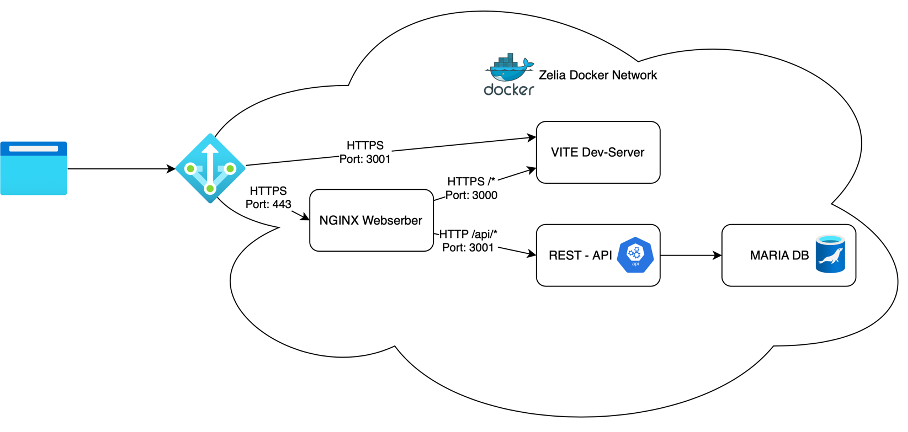
\includegraphics{media/Docker/DevNetwork.png}
    \caption{Docker-Netzwerk für die Entwicklung}
    \label{fig:DockerDevNetwork}
\end{figure}

Um das Datenbankschema aufzubauen und Testdaten einzufügen, können SQL-Skripte im Verzeichnis {\ttfamily /docker-entrypoint-initdb.d/} angelegt werden. Dort werden sie beim Start des Docker-Containers in alphabetischer Reihenfolge ausgeführt. Deshalb wurden die SQL-Skripte durchnummeriert, um die Reihenfolge festzulegen (siehe Abbildung \ref{fig:SQLScriptDir}).

\begin{figure}
    \centering
    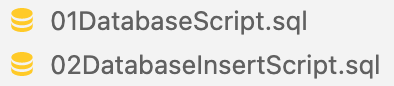
\includegraphics{media/Docker/SQLScriptDir.png}
    \caption{Verzeichnis für SQL-Skripte}
    \label{fig:SQLScriptDir}
\end{figure}

Um "Secrets" wie das Passwort zur Datenbank zu schützen, werden sie aus Umgebungsvariablen übernommen.
Damit es nicht notwendig ist, die Umgebungsvariablen jedes Mal manuell zu setzten, ist es bei Docker mit der Option "{\ttfamily --env-file}" möglich, eine ".env"-Datei anzugeben, die alle Umgebungsvariablen speichert. \label{par:dockerEnvFile} 

\css{code/Docker/dev.yaml}{Docker-YAML für die Entwicklung}
